\chapter{个人总结}

在本次的实验中,我们实现了一个常用却又陌生的底层应用程序 —— Web 服务器。从一开始查看实验指导书到阅读RFC文档,再到研读代码,一步一步走来,完成最终的作品,每一步都能感受到来在 C 这门上古编程语言的魔力与智慧。从一开始惊叹于 yacc 和 lex 的完美配合竟能实现编译器的语法解析,到实现动态数组模块时重新认识 malloc 和 realloc 函数,再到使用 mmap 统一解决文件读取问题进而实现图传,每一次对作品的完善,都是对 C 这门语言的重新理解以及对我们编程思维的提升。

要说最大的收获,可能就是对框架化、模块化编程的理解、站在巨人的肩膀上进步。这次实验无疑为我们提供了一个良好的平台,去钻研、实践所学的书本知识。加深对 HTTP 以及 socket 编程框架的理解。

对我个人而言,结合用 SpringBoot 框架编写 Java 后端程序的经验,我认为我又对计网这个人类智慧的产物有了更加深刻的理解与体会。

\begin{figure}[htbp!]
    \begin{center}
        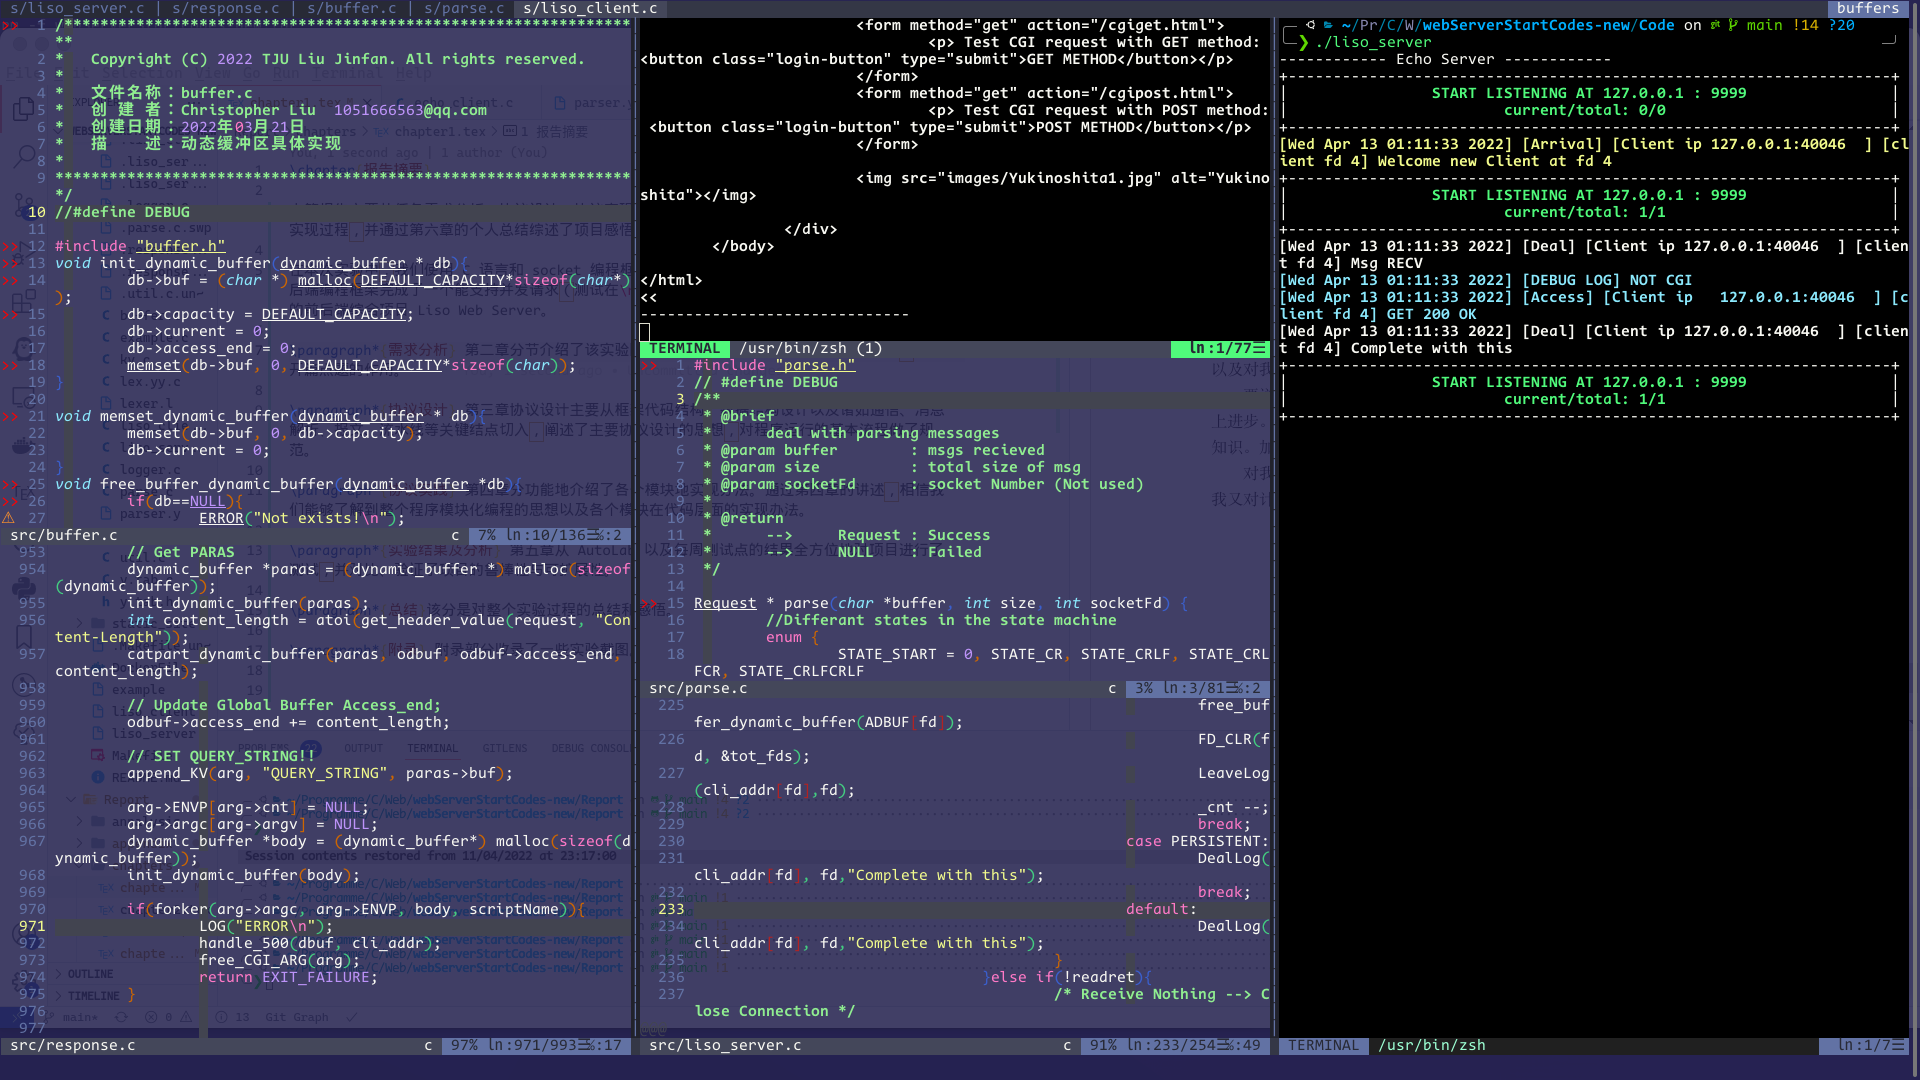
\includegraphics[width=5.5in]{screenshoot1.png}
        \caption{项目测试环境截图}\label{fig:screenshoot1}
    \end{center}
\end{figure}
